\section{Automatic Pipeline Synthesis}
\begin{figure*}[htb]
\centering
  \begin{subfigure}[t]{0.8\textwidth}
  \centering
  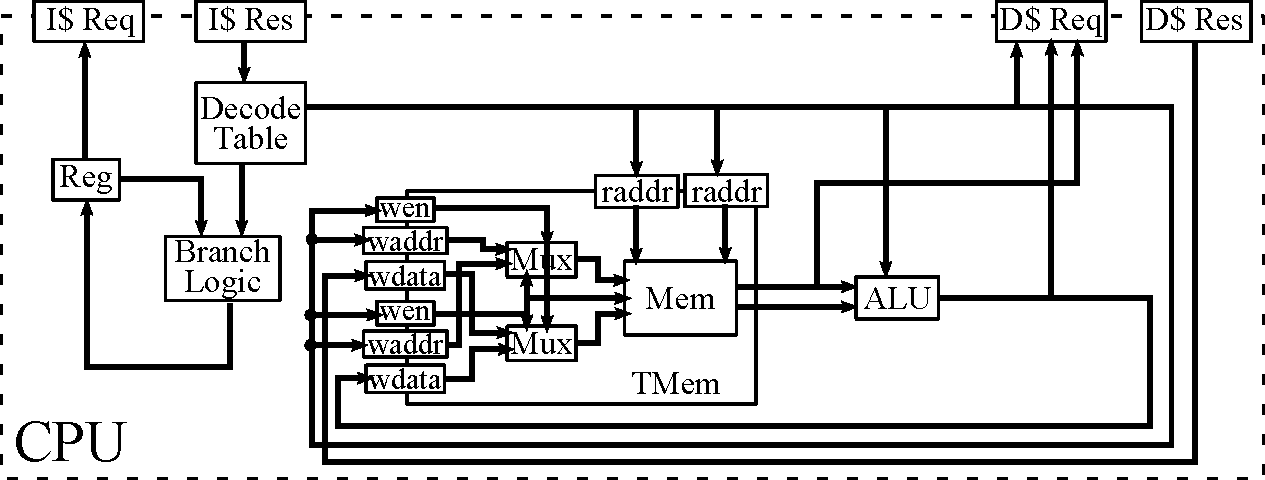
\includegraphics[width=\textwidth]{figures/pipeline.pdf}
  \caption{{\bf Datapath Graph}. CPU datapath represented as a
    directed dataflow graph in Chisel.}
  \label{fig:datapathgrah}
  \end{subfigure}
  \begin{subfigure}[t]{0.8\textwidth}
  \vspace{20pt}
  \centering
  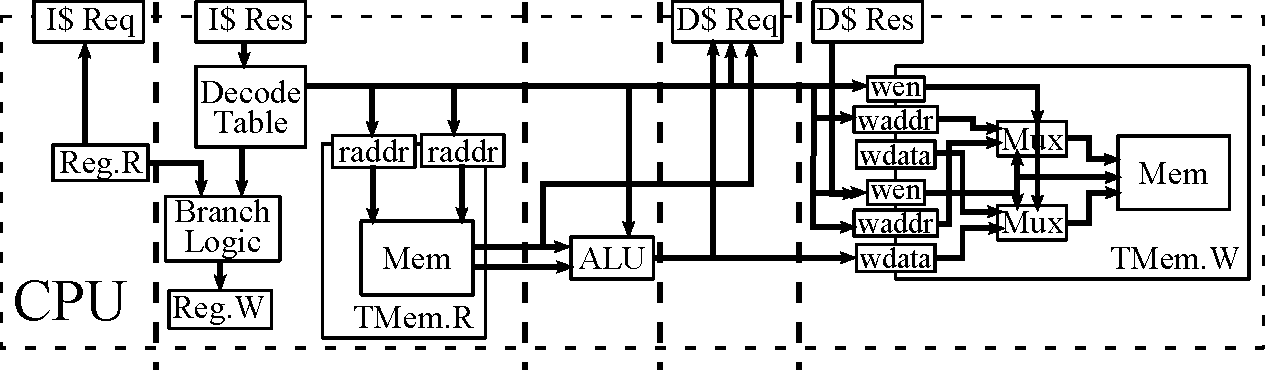
\includegraphics[width=\textwidth]{figures/pipelinedag.pdf}
  \caption{{\bf Datapath DAG}. 5-stage CPU datapath turned into a
    directed acyclic graph by breaking {\tt Reg} nodes and {\tt
      TransactionalMem} into read and write ports. The dashed lines
    represent pipeline boundaries.}
  \label{fig:datapathdag}
  \end{subfigure}
\caption{{\bf 5-stage CPU Datapath}. ALU = arithmetic logic unit. D\$
  = data cache. I\$ =  instruction cache. TMem =
  TransactionalMem. {\tt x}.R = read port of node {\tt x}. {\tt x}.W =
  write port of node {\tt x}}
\label{fig:datapath}
\end{figure*}


\subsection{Pipeline Register Placement and Stage Coloring}


{\bf Pipeline Stage Propagation Details}. 

\begin{figure}[htb]
\centering
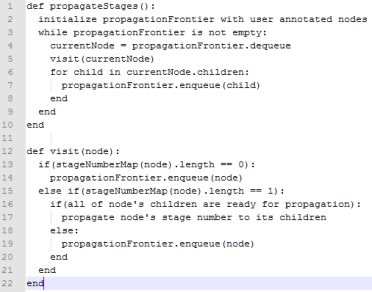
\includegraphics{figures/propagate_pseudo_code.pdf}
\caption{{\bf Pipeline Stage Propagate Pseudo Code}}
\label{fig:propagate}
\end{figure}

\subsection{Hazard Discussion}
\begin{figure*}[htb]
\centering
  \begin{subfigure}[t]{0.8\textwidth}
  \centering
  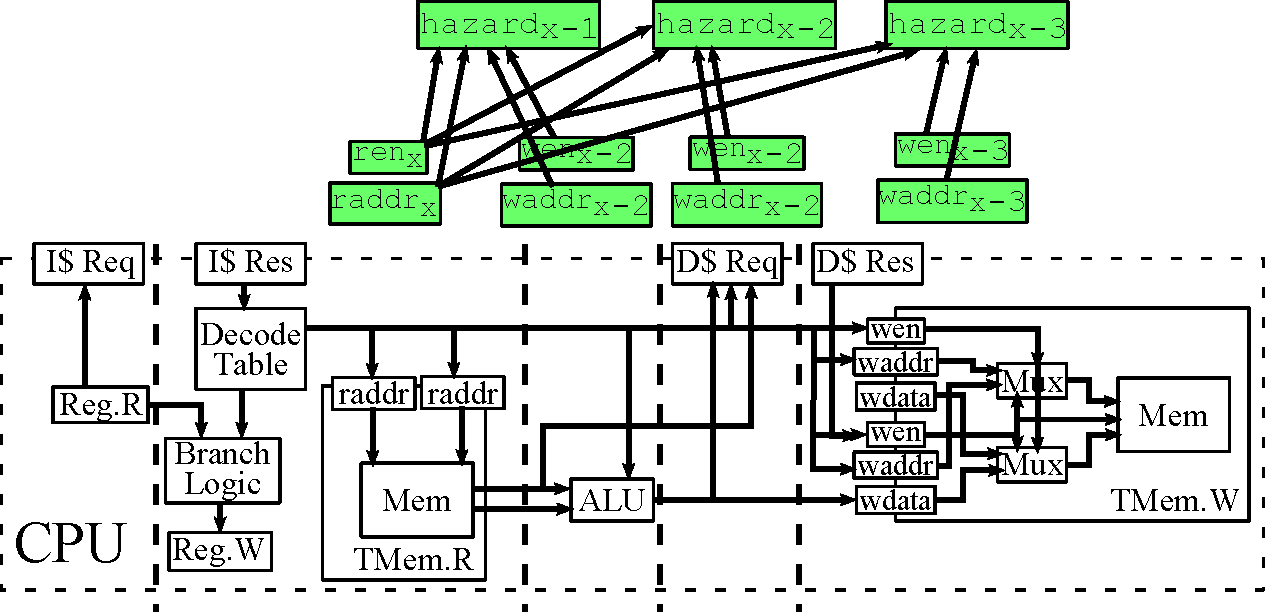
\includegraphics[width=\textwidth]{figures/pipelinehazard.pdf}
  \caption{{\bf Hazard Detection}. All the hazards that
    the {\tt TransactionalMem} generates in a 5-stage pipeline.}
  \label{fig:haz}
  \end{subfigure}
  \begin{subfigure}[t]{0.8\textwidth}
  \vspace{20pt}
  \centering
  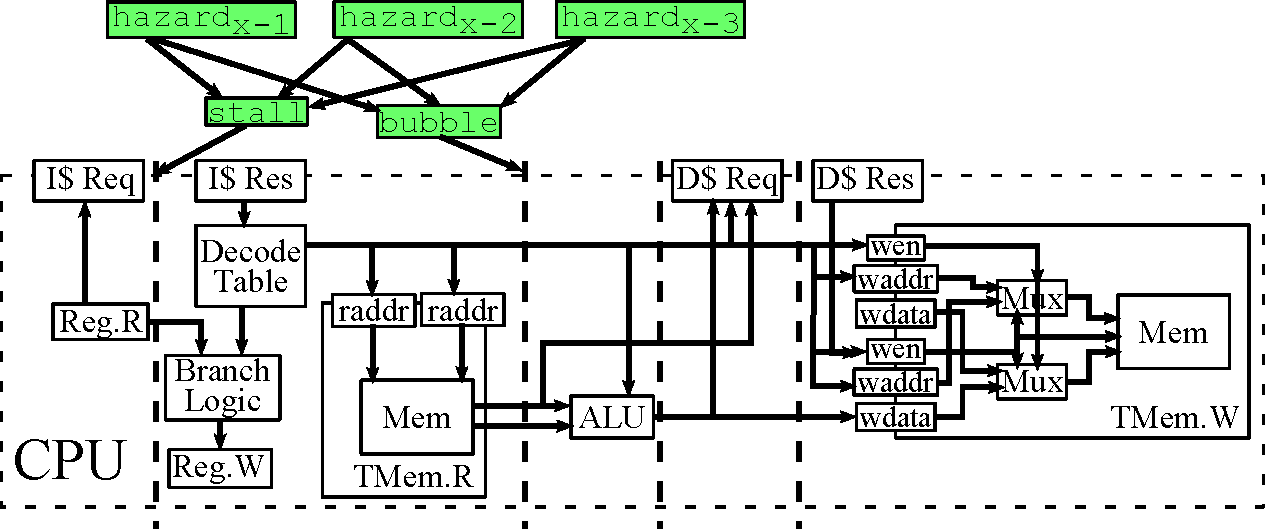
\includegraphics[width=\textwidth]{figures/pipelineinterlock.pdf}
  \caption{{\bf Interlocks}. The hazard conditions stall the
  first and second stage and push bubbles into the third stage.}
  \label{fig:int}
  \end{subfigure}
\caption{Resolving hazards through interlocks.}
\label{fig:hazint}
\end{figure*}

{\bf Hazard Types}. 

\subsection{Hazard Resolution Options}
\begin{figure*}[htb]
\centering
  \begin{subfigure}[t]{0.8\textwidth}
  \centering
  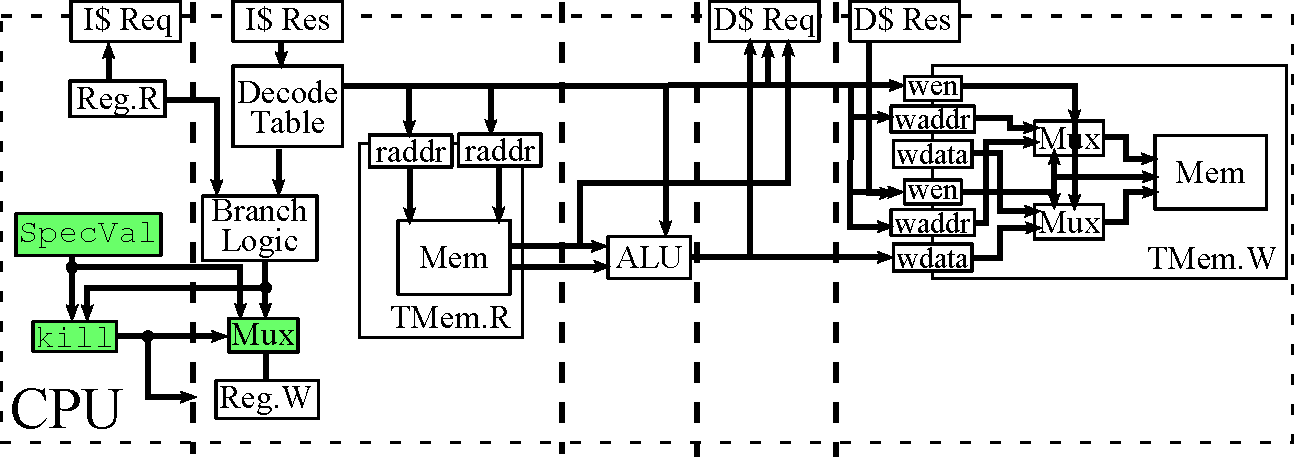
\includegraphics[width=\textwidth]{figures/pipelinespec.pdf}
  \caption{{\bf Speculation}. Using speculation to resolve hazards on
    the {\tt Reg} node whose read port is in the first stage and write port
  is in the second stage.}
  \label{fig:spec}
  \end{subfigure}
  \begin{subfigure}[t]{0.8\textwidth}
  \vspace{20pt}
  \centering
  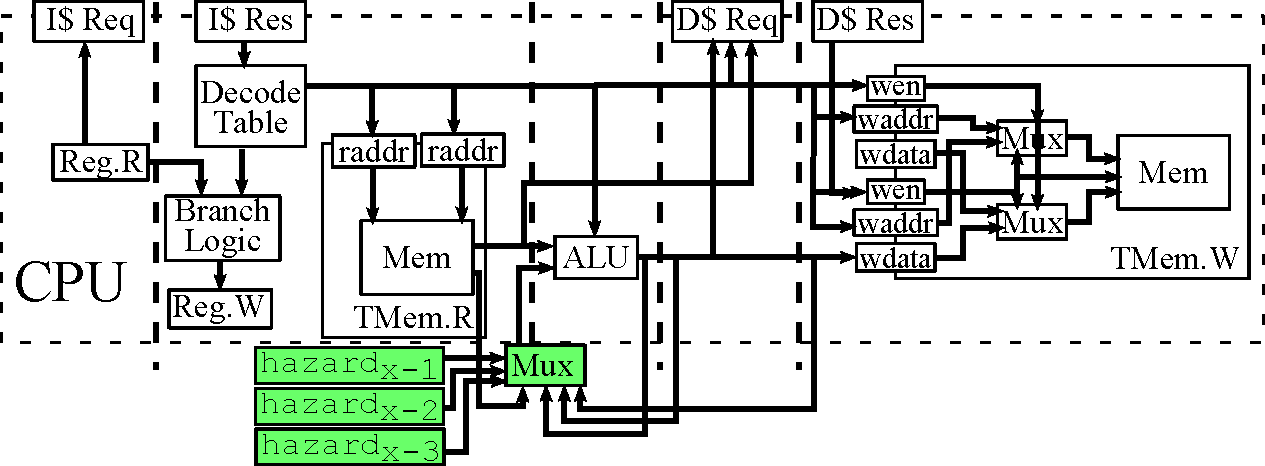
\includegraphics[width=\textwidth]{figures/pipelinebypass.pdf}
  \caption{{\bf Bypassing}. Bypassing network generated to forward ALU
  results from the third stage, fourth stage, and fifth stage to the
  {\tt TransactionalMem}'s second read port.}
  \label{fig:bypass}
  \end{subfigure}
\caption{Resolving hazards through speculation and bypassing.}
\label{fig:specbyp}
\end{figure*}

{\bf Interlocks}. 

{\bf Speculation}. 

{\bf Bypassing}. 

